\documentclass[11pt]{article}
%Gummi|063|=)
\usepackage{amsmath}
\usepackage[authoryear, round]{natbib}
\usepackage{graphicx}
\usepackage{caption}

\title{\textbf{Financial Econometric Models}}
\author{Johannes Degn}
\date{04.02.2014}
\begin{document}

\maketitle

\section{Univariate type-ARCH models}

\section{Multivariate type-ARCH models}
\subsection{}
\subsubsection{BEKK(1,1,1)}
i) \\
$$H_t = C'C + A'\varepsilon_{t-1}\varepsilon_{t-1}'A + B'H_{t-1}B$$
$
H_t = \begin{pmatrix}
c_1 & 0 \\
c_2 & c_3 \\
\end{pmatrix}
\begin{pmatrix}
c_1 & c_2 \\
0 & c_3 \\
\end{pmatrix}
+
\begin{pmatrix}
a_1 & 0 \\
0 & a_2 \\
\end{pmatrix}
\begin{pmatrix}
\varepsilon_{t-1, 1} \\
\varepsilon_{t-1, 2} \\
\end{pmatrix}
\begin{pmatrix}
\varepsilon_{t-1, 1} & \varepsilon_{t-1, 2} \\
\end{pmatrix}
\begin{pmatrix}
a_1 & 0 \\
0 & a_2 \\
\end{pmatrix}
+
\begin{pmatrix}
b_1 & 0 \\
0 & b_2 \\
\end{pmatrix}
\begin{pmatrix}
h_{t-1, 11} & h_{t-1, 12} \\
h_{t-1, 21} & h_{t-1, 22} \\
\end{pmatrix}
\begin{pmatrix}
b_1 & 0 \\
0 & b_2 \\
\end{pmatrix}
$
\\
\\
\noindent
\\
$
H_t = \begin{pmatrix}
c_1^2 & c_1c_2 \\
c_1c_2 & c_2^2+c_3^2 \\
\end{pmatrix}
+
\begin{pmatrix}
a_1^2\varepsilon_{t-1, 1}^2 & a_1a_2\varepsilon_{t-1, 1}\varepsilon_{t-1, 2} \\
a_1a_2\varepsilon_{t-1, 1}\varepsilon_{t-1, 2} & a_2^2\varepsilon_{t-1, 2} \\
\end{pmatrix}
+
\begin{pmatrix}
b_1^2h_{t-1, 11} & b_1b_2h_{t-1, 12} \\
b_1b_2h_{t-1, 21} & b_2^2h_{t-1, 22} \\
\end{pmatrix}
$
\\
\\
\noindent $h_{t, 11}$, $h_{t, 22}$ and $h_{t, 12}$ can be read from the respective addition above.
\\
\\
\noindent
ii)
positivity constraints are satisfied as the diagonal elements ($h_{t, 11}$ and $h_{t, 22}$) are bigger than or equal to 0. TODO: CHECK THIS WHAT IS ASKED! \\
\\
iii) 
\begin{figure}[hc]
\centering
\caption{Simulated series of a BEKK(1,1,1)}
\caption*{parameters: $A = \begin{pmatrix} 
0.5 & 0 \\
0 & 0.5 \\
\end{pmatrix}$, $B = \begin{pmatrix} 
0.5 & 0 \\
0 & 0.5 \\
\end{pmatrix}$, $C = \begin{pmatrix} 
1 & 1 \\
0 & 1 \\
\end{pmatrix}$}
\label{correlogram1}
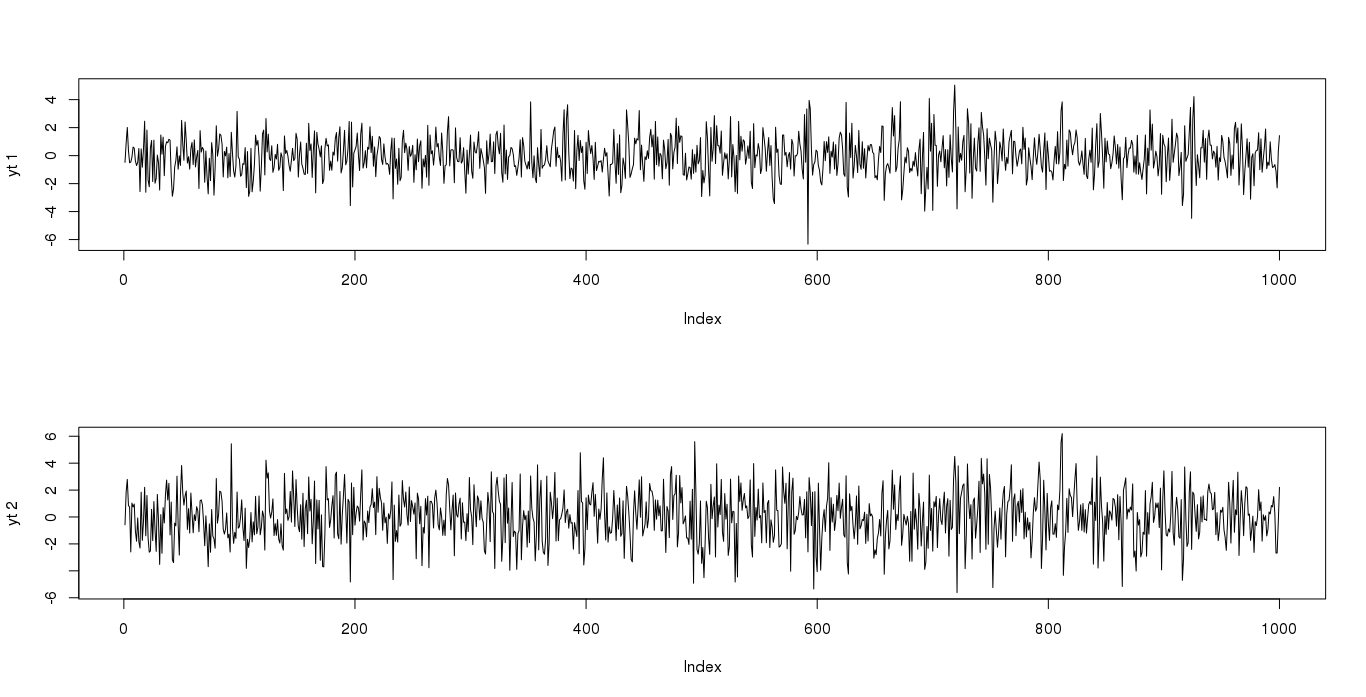
\includegraphics[width=160mm]{graphs/problem2_simulated_series.png}
\end{figure}
\clearpage

\subsection{}
a) \\
\\
\\
b) \\
With $CC' = I_2CC'$ and $vec(A+B) = vec(A) + vec(B)$ follows: \\
$vec(\Sigma_t) = vec(CC') + vec(B\Sigma_{t-1}B') + vec(A\varepsilon_{t-1}\varepsilon_{t-1}'A')$ \\ $ = (C \otimes I_2 )vec(C) + (B \otimes B)vec(\Sigma_{t-1}) + (a \otimes A)vec(\varepsilon_{t-1}\varepsilon_{t-1}')$
\\
\\
Note that since the off-diagonal elements of $\Sigma_t$ are identical we could use the half-vectorization leaving out one of the two off-diagonal elements without losing information.
\\
\\
c) \\
The intercept vector is given by $(\hat C \otimes I_2)vec(\hat C) = \begin{pmatrix} 0.0225 \\ 0.0285 \\ 0.0285 \\ 0.0761 \\ \end{pmatrix}$
\\
\\
d) \\
Exceedance correlations are correlation coefficients computed for return values above a threshold parameter $\theta$ (here $\theta$ is denoted in quantiles of the data). Exceedance correlations can be used to calculate conditional correlation. They capture assymetrie in the tail dependence (i.e. different dependence between high and low value returns). Empirical data on stock returns show asymmetric correlations while simple models which use e.g. multivariate normally distributed error terms or GARCH errors can not reproduce this behaviour. \citet{ang2002international} use show that regime switching models can reproduce asymmetric correlations.
\\
\\
e) \\
The figure shows conditional correlation coefficients between returns of S\&P 500 and FTSE 100 indices for two different time periods: 1984-1989 and 2000-2008. While for the period of 2000-2008 the exceedance correlations appear to be relatively stable with respect to the threshold parameter, the period of 1984-1989 shows a strong asymmetrie of correlation coefficients. Returns above the 50-percentile show a lower correlation. The correlation of returns off the two indices start growing again above the 70-percentile.
\bibliographystyle{plainnat}
\bibliography{/home/joi/workspace/latex/citations}
\end{document}
